\section{案例分析与可视化}

\subsection{四个代表词的频谱模板}

图~\ref{fig:matlab-spectra} 给出了四个代表词在 MATLAB 演示中的短时 FFT 模板，用来直接观察这些局部谱形的基本形状。

\begin{figure}[H]
    \centering
    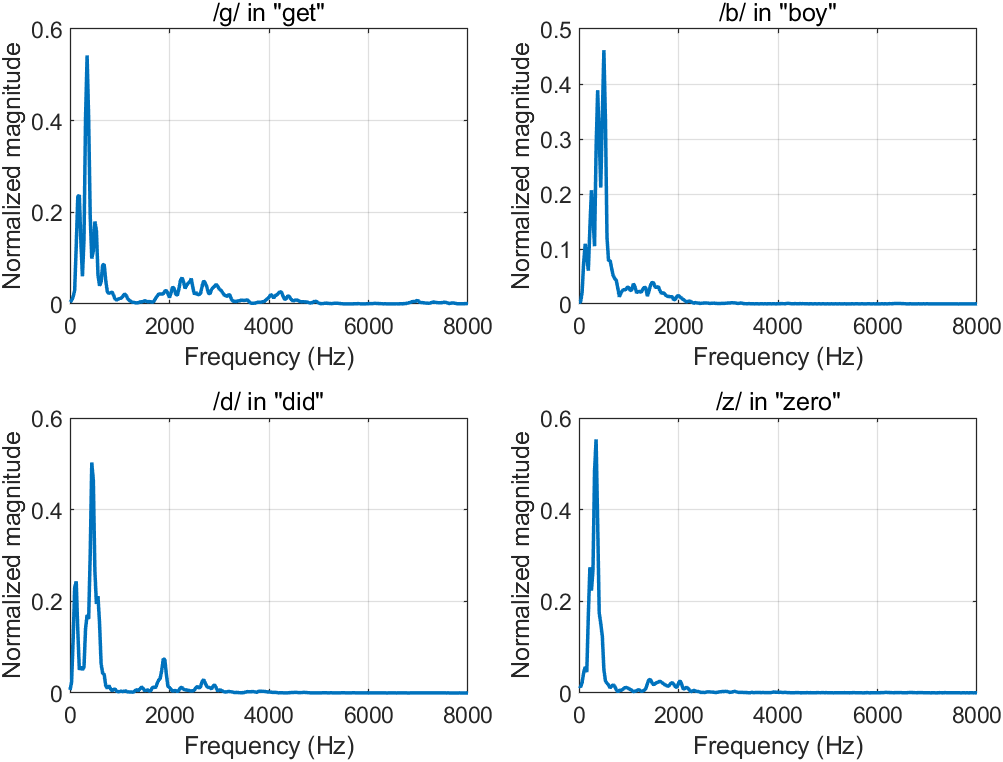
\includegraphics[width=0.95\textwidth]{figures/course_matlab/example_short_time_spectra.png}
    \caption{四个代表词的短时 FFT 幅度谱模板。}
    \label{fig:matlab-spectra}
\end{figure}

从图上能直接看出，/z/ 的高频摩擦更连续，/b/ 和 /d/ 的起始爆破更短，/g/ 的短时结构最容易被时间对齐误差冲掉。这个结论和模板构造图是一致的。

\subsection{相关得分矩阵}

图~\ref{fig:matlab-score} 给出了同一组模板在四个案例词上的相关得分矩阵，展示了局部语音片段与模板之间的对应关系。

\begin{figure}[H]
    \centering
    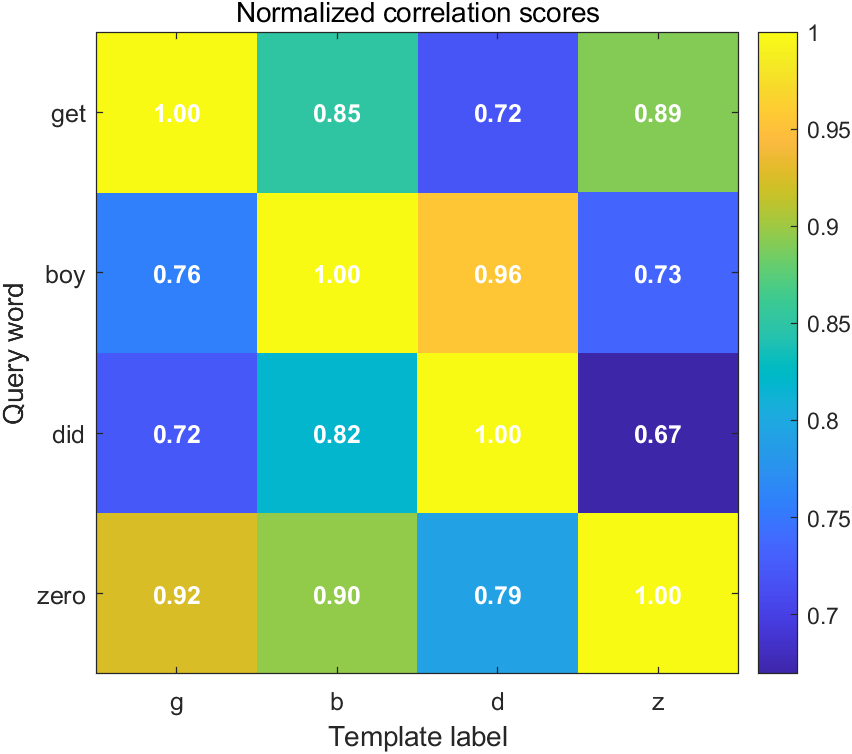
\includegraphics[width=0.70\textwidth]{figures/course_matlab/example_score_matrix.png}
    \caption{四个代表词对应的相关得分矩阵。}
    \label{fig:matlab-score}
\end{figure}

这个矩阵比单纯看波形更直接，因为它把“哪个模板更像这段语音”变成了数值。如果相关分数差距不大，就说明这个词首辅音对齐还不够稳，这也是后文基于 AI 的重实现方法要解决的问题。
